% additional use of \usepackage{beamerthemesplit}
\documentclass{beamer}
\usepackage{beamerthemesplit} % new 
\usepackage{hyperref}
\usepackage{multimedia}
\usetheme{Frankfurt}
\definecolor{verde}{rgb}{0.5,1,0.2}
\definecolor{rojo}{rgb}{1,0,0}

\begin{document}
\title{The Merging Systems Identification (MeSsI) Algorithm.} 
\author{Mart\'in de los Rios, Mariano Dom\'inguez, Dante Paz} 

\frame{\titlepage
\date{}} 

\frame{
 \tiny
 \frametitle{Table of contents}
\tableofcontents} 

\section{Why searching merging galaxy clusters?}
\frame{
\tableofcontents[ 
    currentsection, 
    hideothersections, 
    sectionstyle=show/hide, 
    sectionstyle=show/shaded, 
    ] 
}

\subsection{Study dark matter particle properties.}

\frame{
 \frametitle{You can study dark matter particle properties}
 \begin{figure}[!b]
  \centering
  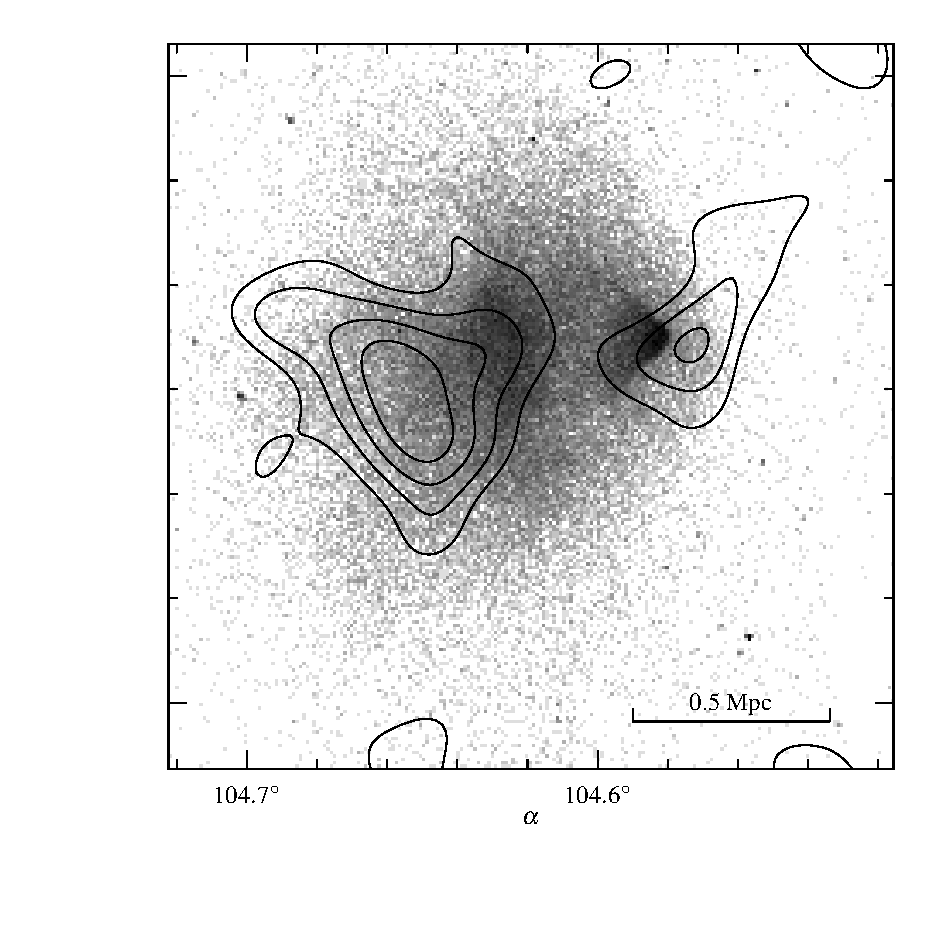
\includegraphics[scale=0.25]{./1e_xrayimg_lens_sm7.eps}
  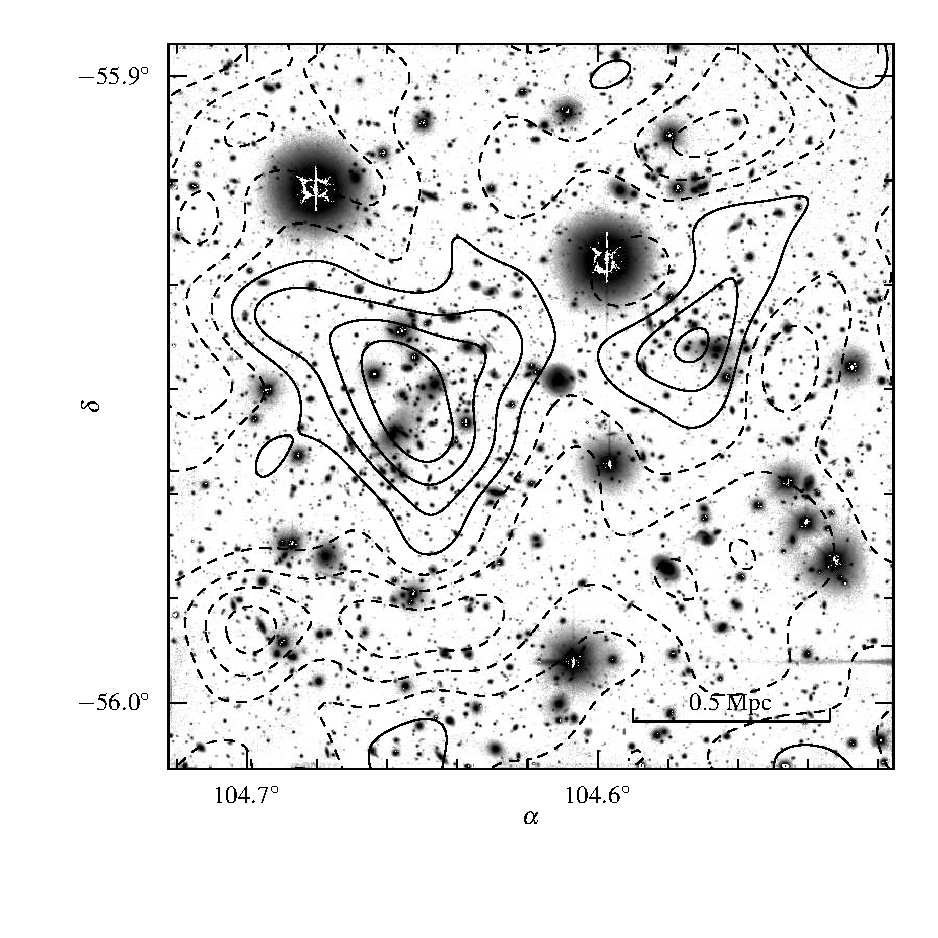
\includegraphics[scale=0.25]{./1e_optvlt_lens_sm7.eps}
 % 1e_optvlt_lens_sm7.eps: 0x0 pixel, 300dpi, 0.00x0.00 cm, bb=0 0 434 434
 \end{figure}
}

\frame{
 \frametitle{Markevitch et al. 2004}
 \begin{itemize}
  \item Desfasaje entre la materia oscura y el gas:
 \end{itemize}

 $ \tau_{s}=\frac{\sigma}{m} \Sigma_{s} $ 
 donde $\sigma$ es la secci\'on eficaz, \textit{m} es la masa de la part\'icula y $\Sigma_{s}$ es la densidad superficial de DM.
 La densidad superficial promediada dentro de $r = r_{tr}$ es $\Sigma \approx 0.2 g cm^{-2}$,
 entonces, asumiendo simetr\'ia esf\'erica y pidiendo que $\tau_{s}<1$ tenemos: $\frac{\sigma}{m} < 5 cm^{2}g^{-1}$.
 \begin{table}
 \begin{tabular}{|c|c|}
  \hline
  C\'umulo & $\frac{\sigma}{m}$ \\
  \hline \hline
  Bullet Cluster & $< 5 cm^{2}/g$ \\
  Musket Ball & $<7 cm^{2}/g$ \\
  Baby Bullet & $<4 cm^{2}/g$ \\
  \hline
 \end{tabular}
 \end{table}
}

\frame{ 
 \begin{itemize}
  \item La gran velocidad del c\'umulo secundario:
 \end{itemize}

 \begin{figure}[h!]
  \centering
  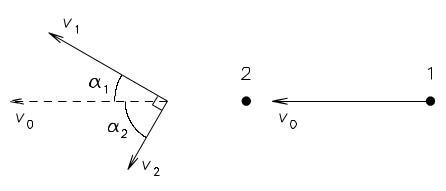
\includegraphics[scale=0.35]{./colision.png}
 % colision.png: 446x191 pixel, 72dpi, 15.73x6.74 cm, bb=0 0 446 191
 \end{figure}
 \begin{tiny}
 \begin{eqnarray}
  \bar{p} & = & mv_{s} \left[ 1-4\int_{sen\alpha_{c}}^{1} x^{2} \left( x^{2}-\frac{V^{2}}{v^{2}}(1-x^{2}) \right)^{1/2} dx \right] \approx 0.1 mv_{s} \\
    %n & = & \frac{M_{s}}{m}\frac{\sigma}{m} \rho_{m} v \\
    \frac{d(v-v_{ff})}{dt} & = &  \frac{\bar{p}n}{M_{s}}=\frac{\bar{p}}{m}\frac{\sigma}{m}\rho_{m}v \\
    v-v_{ff} & = & \frac{\bar{p}}{m}\frac{\sigma}{m} \Sigma_{m} \\
    v-v_{ff} &<& 1000 km/s \\
    \frac{\sigma}{m} & < & 7cm^{2}/g
 \end{eqnarray}
 \end{tiny}
}

\frame{
 \begin{itemize}
  \item La supervivencia del c\'umulo secundario.
 \end{itemize}
 \begin{eqnarray}
  \chi&=&1-2\frac{v^{2}_{esc}}{v_{0}^{2}} \\
   \tau_{m}&=&\frac{\sigma}{m}\Sigma_{m} \\
    \chi \tau_{m}&=&\frac{\sigma}{m}\Sigma_{m} \left[ 1-2 \frac{v_{esc}^{2}}{v_{0}^{2}} \right] \\
    \chi \tau_{m}&<&0.3 \\
     \frac{\sigma}{m}& < &1 cm^{2}/g
 \end{eqnarray}
}


\frame{ 
 \frametitle{Harvey et al. 2015}
 \begin{figure}[h!]
 \centering
 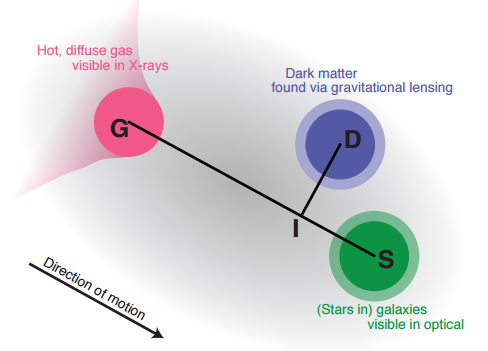
\includegraphics[scale=0.3]{./massey1.png}
 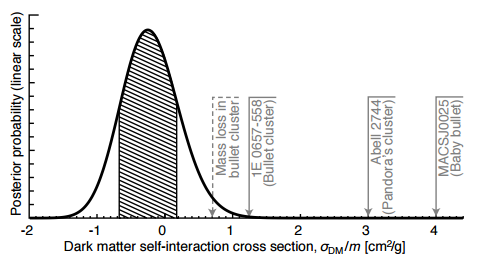
\includegraphics[scale=0.3]{./massey2.png}
\end{figure}
$\frac{\sigma}{m} \leq 0.47 cm^{2}/g$
}

\subsection{Test cosmological models.}
\frame{ 
 \frametitle{You can test your favourite cosmological model.} 
 \begin{itemize}
  \item Estudio de la probabilidad de que un c\'umulo tenga una velocidad similar a la del bullet cluster. 
   \begin{itemize}
    \item Hayashi et al. 2006
    \item Farrar y Rosen 2007
    \item Lee y Komatsu 2010
    \item Forero-Romero et al. 2010
    \item Thompson y Nagamine 2011
    \item Watson et al. 2013
   \end{itemize}
  \item Estudios con simulaciones hidrodin\'amicas
    \begin{itemize}
     \item Springel \& Farrar. 2005
     \item Milosavljevic et al. 2007
     \item Mastropietro \& Burket. 2008
     \item Lage \& Farrar 2014
    \end{itemize}
 \end{itemize}
}

\frame{
 \frametitle{The Rise and Fall of a challenger by Thompson (2014).}
 \begin{itemize}
  \item They investigate the probability of finding such a high-velocity pair in 
   large-volume N-body simulations, particularly focusing on differences between halo finding algorithms.
  \item  When employing the Rockstart (Behroozi et al 1013) halo finder that considers particle velocities, they find
   numerous Bullet-like pair candidates that closely match not only the high pairwise velocity, 
   but also the mass, mass ratio, separation distance, and collision angle that have been shown to produce the Bullet Cluster.
  \item The probability of finding a massive, high pairwise velocity pair
   among halos with $M_{\rm halo}\geq10^{14} M_\odot$ is $4.6\times 10^{-4}$
   using RS, while it is $\approx 45\times$ lower using a friends-of-friends (FOF) based approach as in previous studies.
 \end{itemize}
}


\frame{
 \frametitle{High velocity tail of Bullet like pairs.}
 \begin{figure}[h!]
  \centering
  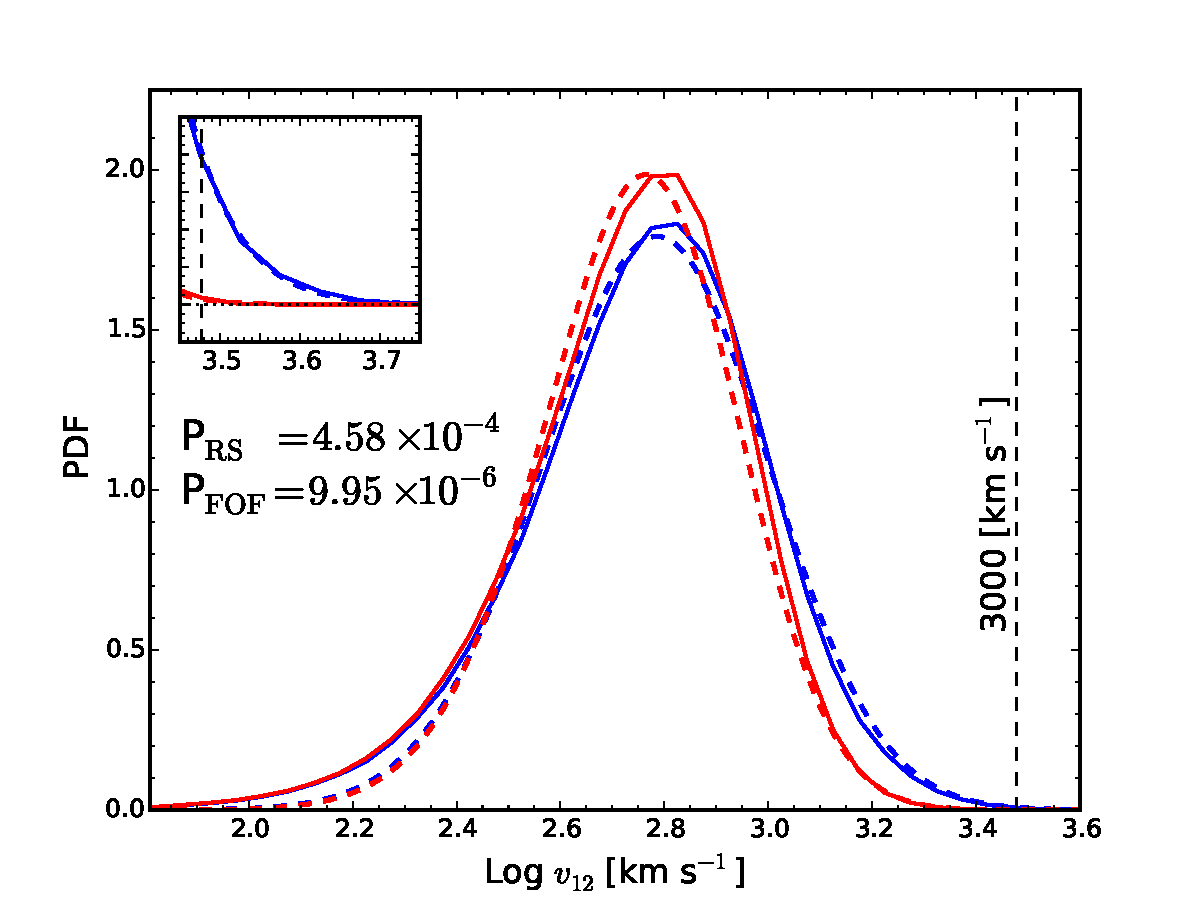
\includegraphics[scale=0.3]{./figure3.pdf}
 % mill.png: 555x565 pixel, 72dpi, 19.58x19.93 cm, bb=0 0 555 565
  \caption{Probability distribution function of massive halo pairs in 
   largest simulation (L4500) identified by FOF (Red solid line) and RS (Blue solid line).}
 \end{figure}
}

\subsection{Study Intra-Clusters Medium properties.}
\frame{
 \frametitle{You can study the ICM properties.}
 
  \begin{figure}[h!]
 \centering
 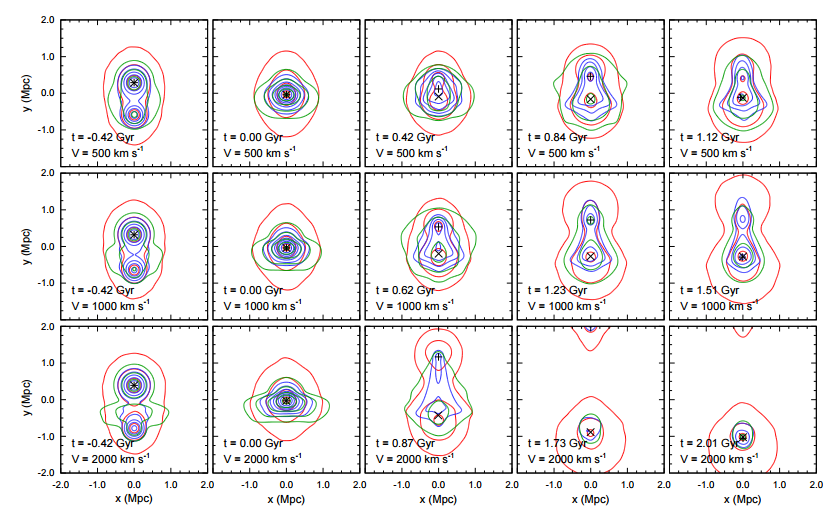
\includegraphics[scale=0.35]{./sz1.png}
 % sz1.png: 1003x598 pixel, 72dpi, 35.38x21.10 cm, bb=0 0 1003 598
 \caption{Zhang et al. 2014}
\end{figure}

}

\section{The MeSsI Algorithm}
\frame{
\tableofcontents[ 
    currentsection, 
    hideothersections, 
    sectionstyle=show/hide, 
    sectionstyle=show/shaded, 
    ] 
}

%\frame{
 %\frametitle{Other approachs for merging clusters detection}
 %\begin{columns}
  %\begin{column}{5cm}
   %Radio Haloes
  %\end{column}
  %\begin{column}{5cm}
   %X-ray morphologies
  %\end{column}
 %\end{columns}
%}

\frame{
 \begin{figure}[h!]
  \centering
  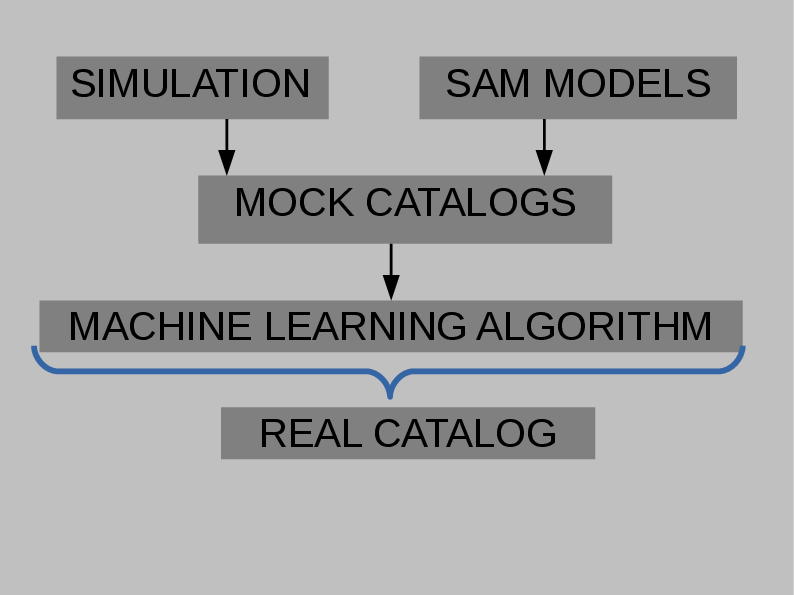
\includegraphics[scale=0.3]{./resu.png}
 % resu.pdf: 794x595 pixel, 72dpi, 28.01x20.99 cm, bb=0 0 794 595
 \end{figure}
}


\frame{ \frametitle{Clusters identification.}
\begin{itemize}
 \item We construct a mock catalogue based on the results of the application of the SAM Model of Guo et al. 2010
  to the Millenium simulation. \pause
 \item We Perform a friend-of-friend algorithm (\textit{Merchan \& Zandivares 2002 }) to the mock catalog in order to identify
  the clusters. \pause
 \item We assign each identified cluster with a fof-group in the simulation.
\end{itemize}
}

\frame{\frametitle{Study of the merger trees.}
 \begin{itemize}
  \item Based on the subhalos merger trees, we construct the merger tree for every fof group in the simulation.
 \end{itemize}
 \begin{figure}[h!]
  \centering
  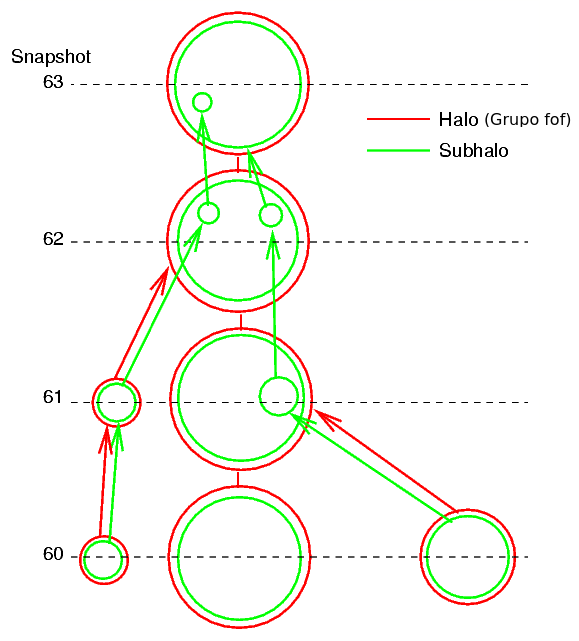
\includegraphics[scale=0.32]{./tree.png}
 % tree.eps: 0x0 pixel, 300dpi, 0.00x0.00 cm, bb=14 14 554 655
 \end{figure}
}

\subsection{Machine learning algorithm applied for identification of substructures.}


\frame{
 \begin{columns}
  \begin{column}{5cm}
   \begin{itemize}
    \item Dressler-Shectman test.
    \item Non gaussianity test.
    \item Color.
    \item Number of galaxies.
   \end{itemize}
  \end{column}
  \begin{column}{5cm}
   \begin{figure}[h!]
    \centering
    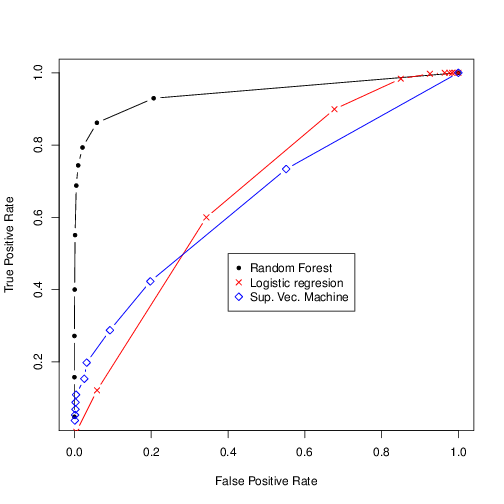
\includegraphics[scale=0.3]{./roc_curves.png}
    % roc_curves.pdf: 504x504 pixel, 72dpi, 17.78x17.78 cm, bb=0 0 504 504
   \end{figure}
  \end{column}
 \end{columns}
}

\frame{
\begin{figure}[h!]
 \centering
 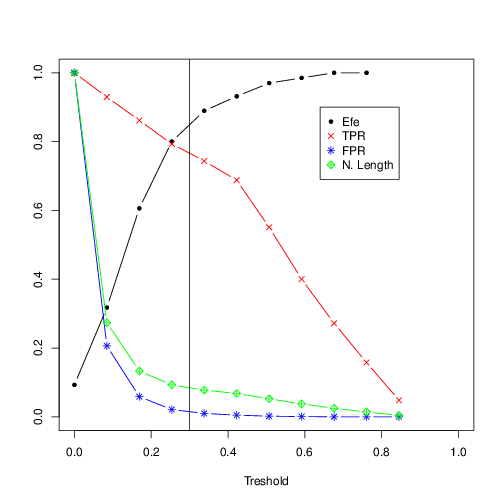
\includegraphics[scale=0.3]{./treshold.png}
 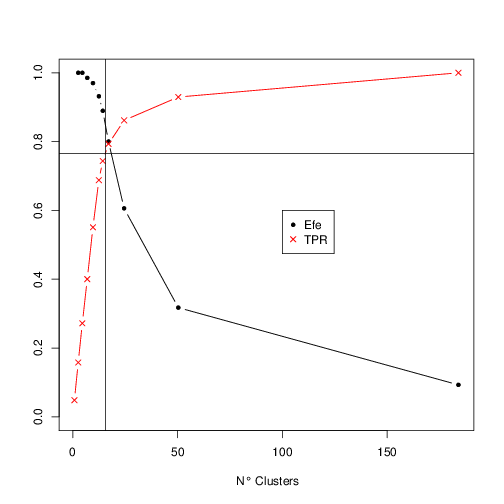
\includegraphics[scale=0.3]{./ncluster.png}
 % treshold.pdf: 504x504 pixel, 72dpi, 17.78x17.78 cm, bb=0 0 504 504
\end{figure}

}

\frame{
\frametitle{Study of the identified substructures.}
\begin{tiny}
\begin{itemize}
 \item We ran a second stage of a random forest algorithm, applied to the galaxies. \pause
 \item In order to define substructures we identify clumps of galaxies based on their proximity, using a
  mixture of gaussians weighted by the probability of each galaxy of being part of a substructure, calculated
  with the RF. \pause
 \item After the substructure identification, each one was related with the subhalo in the mock that have more galaxies in the group identified by
  mclust. \pause
 \item After that, we estimate the velocity dispersion and the virial radius.
  \begin{eqnarray} \label{rvir_disp}
   R_{vir} & = & \frac{\pi}{2} \frac{ngal(ngal-1)}{\sum_{i>j}^{ngal}R_{ij}^{-1}} \nonumber\\
   \sigma &=& \frac{\sqrt{\pi}}{ngal(ngal-1)} \sum_{i=1}^{ngal-1} \omega_{i} g_{i} \nonumber\\
   \omega_{i} &=& i(ngal-i) \nonumber\\
   g_{i} &=& v_{i+1}-v_{i} \nonumber\\ 
  \end{eqnarray}
\end{itemize}
\end{tiny}
}

\frame{
\frametitle{Study of the identified substructures.}
\begin{itemize}
 \item We compare the center of the identified substructures with the centers of the associated subhalos, finding a good estimation. \pause
 \item We compare the virial radius of the identified substructures with the virial radius of the subhalos, finding that we are overestimating the real values. \pause
 \item We compare the velocity dispersion of the identified substructures with the velocity dispersion of the associated subhalos, finding that our values are
  in good concordance with the real values. 
\end{itemize}
}

\frame{
\begin{tiny}
 

With this association between substructure and subhalos in the mock, we find 3 cases:

\begin{enumerate}
\item Clusters where we identify the type 0 subhalo (the principal subhalo of the fof group) and a type 1 subhalo. \pause
\item Clusters where we identify two type 1 subhalos. \pause
 \item Clusters where Mclust find two substructures that are associated to the same type 0 subhalo. \pause
\end{enumerate}
\end{tiny}

\begin{figure}[h!]
 \centering
 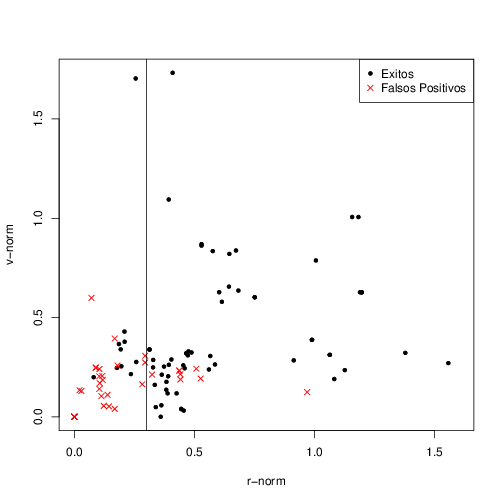
\includegraphics[scale=0.33]{./vnorm_rnorm.png}
 % vnorm_rnorm.pdf: 504x504 pixel, 72dpi, 17.78x17.78 cm, bb=0 0 504 504
\end{figure}

}

\frame{
 \frametitle{Mock Clusters}
 \begin{columns}
  \begin{column}{3cm}
   \begin{figure}[h!]
    \centering
    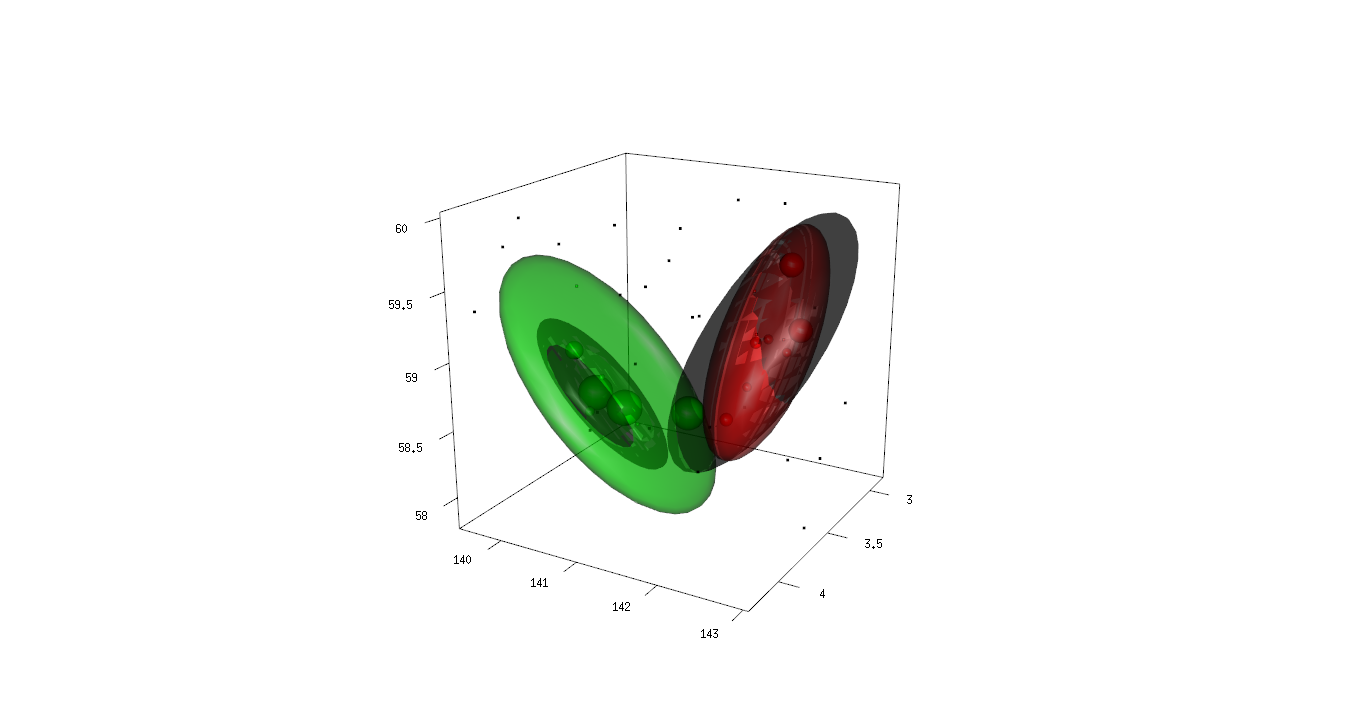
\includegraphics[scale=0.2]{./3619_fig3.png}
 % 42552_fig3.png: 1360x712 pixel, 72dpi, 47.98x25.12 cm, bb=0 0 1360 712
   \end{figure}
  \end{column}
  \begin{column}{3cm}
   \begin{figure}[h!]
    \centering
    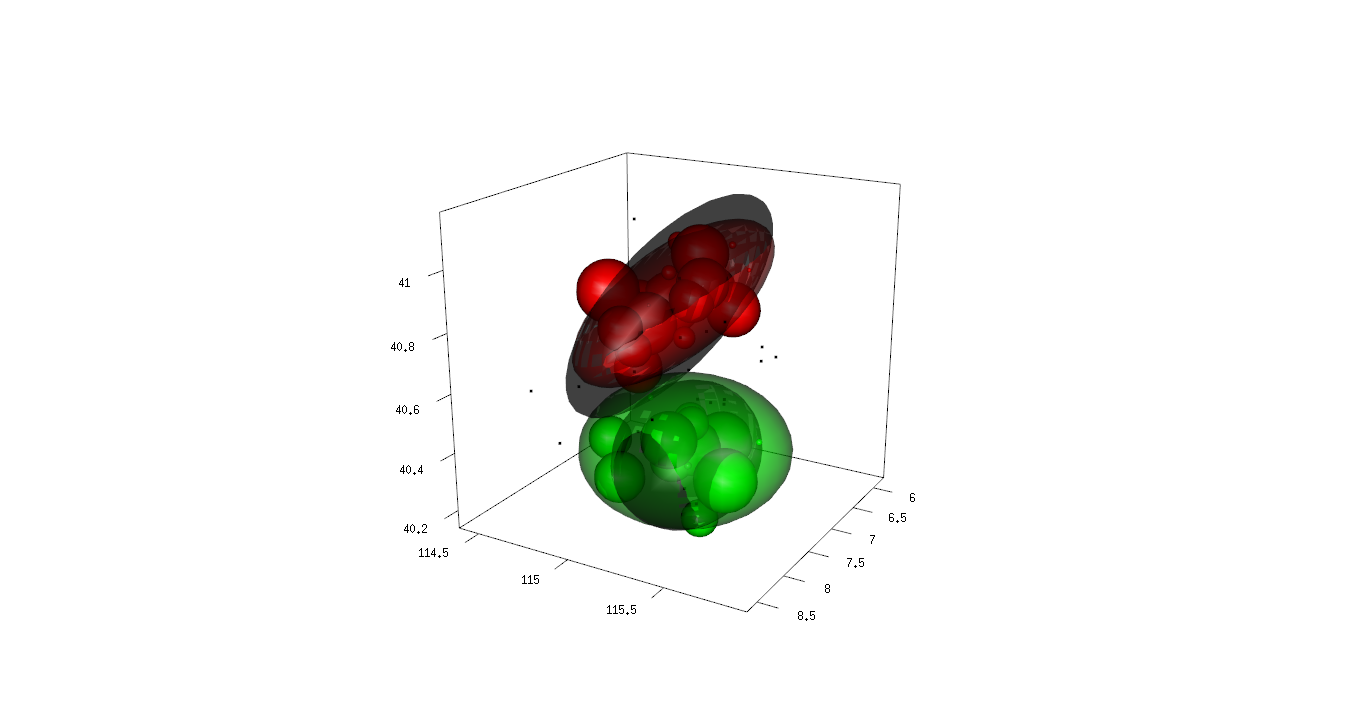
\includegraphics[scale=0.2]{./10514_fig3.png}
 % 94314_a1991_fig3.png: 1360x712 pixel, 72dpi, 47.98x25.12 cm, bb=0 0 1360 712
  \end{figure}
  \end{column}
 \end{columns}
}

\subsection{Application of the MeSsI Algorithm to spectroscopy catalogues}
\frame{
 \frametitle{Application of the MeSsI Algorithm to spectroscopy catalogues}
  \begin{itemize}
   \item We find 12 Clusters with high probability of been in a merger in the SDSS DR7.
  \end{itemize}

  Abell 1991
  \begin{figure}[h!]
   \centering
   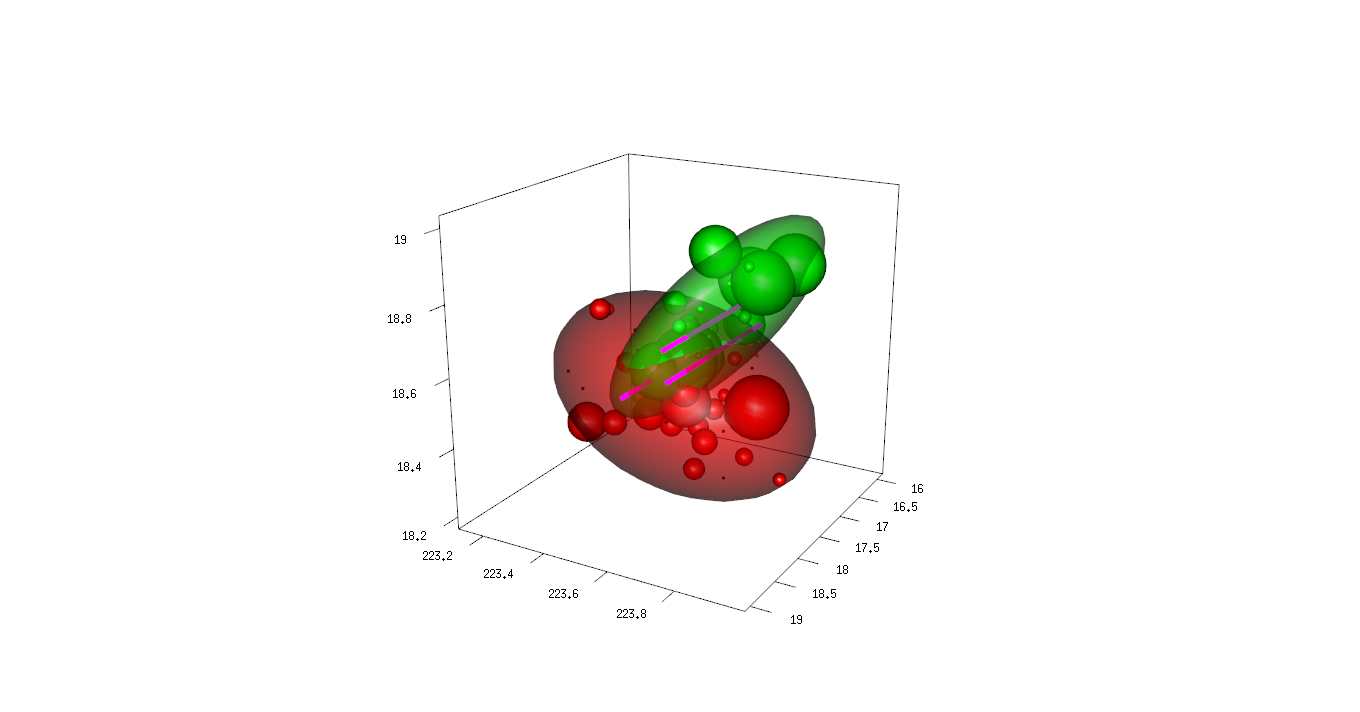
\includegraphics[scale=0.2]{./94314_a1991_fig3.png}
 % 94314_a1991_fig3.png: 1360x712 pixel, 72dpi, 47.98x25.12 cm, bb=0 0 1360 712
  \end{figure}
}
\frame{
 \begin{itemize}
   \item We find 7 Clusters with high probability of been in a merger in the WINGS Clusters.
 \end{itemize}

 \begin{figure}[h!]
  \centering
  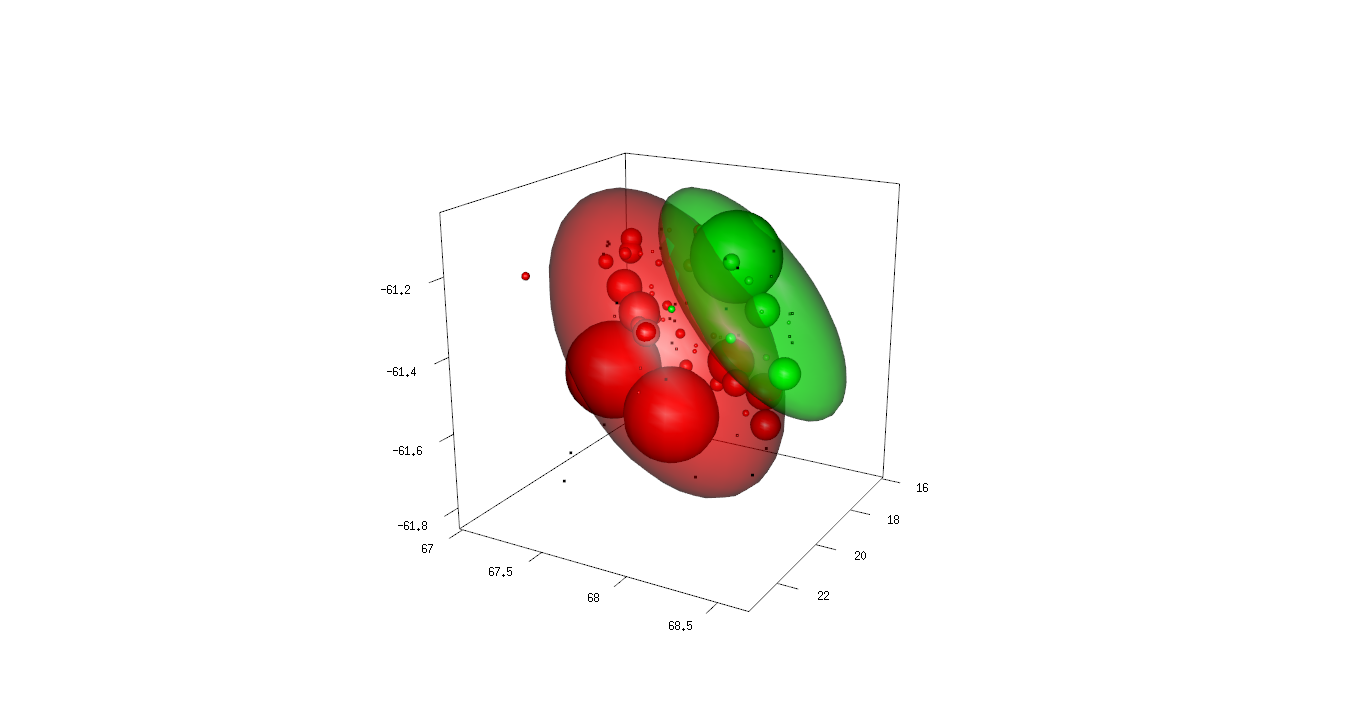
\includegraphics[scale=0.2]{./15_a3266_fig3.png}
 % 94314_a1991_fig3.png: 1360x712 pixel, 72dpi, 47.98x25.12 cm, bb=0 0 1360 712
 \end{figure}

}
\frame{
 \begin{itemize}
   \item We find 15 Clusters with high probability of been in a merger in the HECs Clusters.
 \end{itemize}

 Abell 2631
 \begin{figure}[h!]
  \centering
  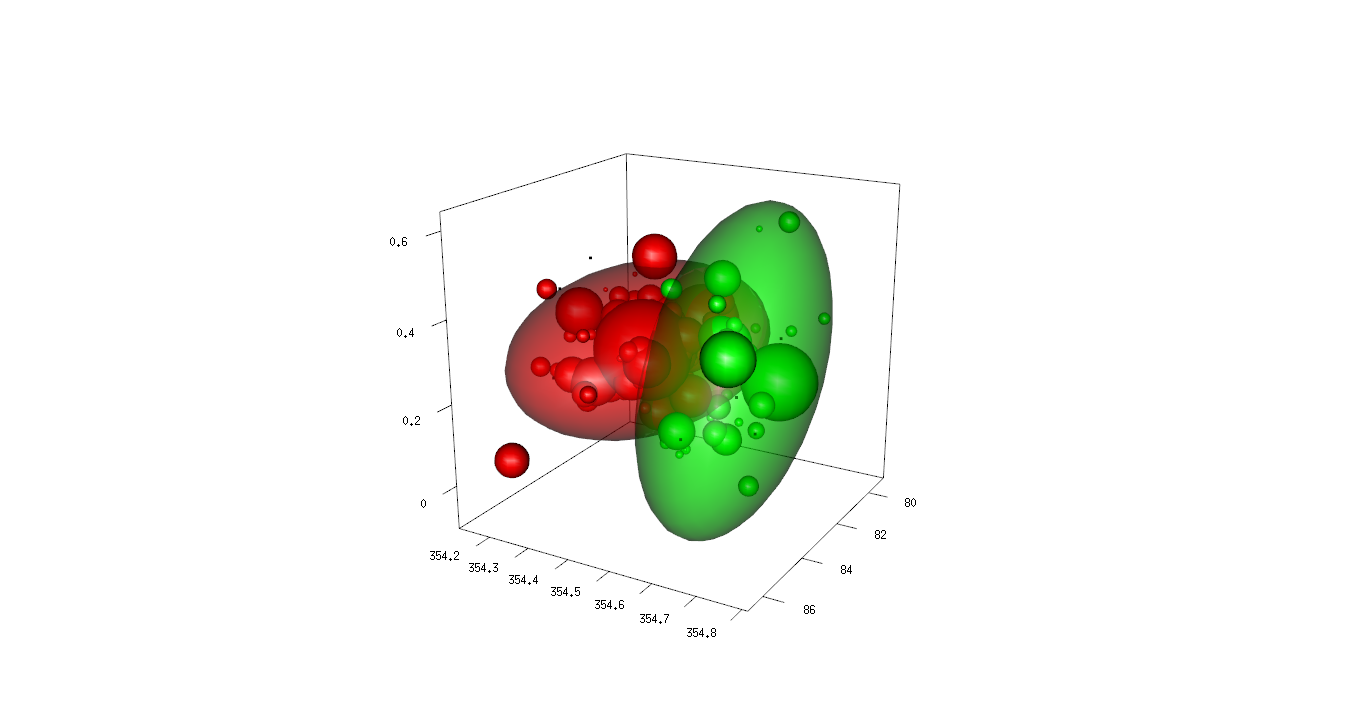
\includegraphics[scale=0.2]{./57_a2631_fig3.png}
 % 94314_a1991_fig3.png: 1360x712 pixel, 72dpi, 47.98x25.12 cm, bb=0 0 1360 712
 \end{figure}

}

\section{Future Work}
\frame{
\tableofcontents[ 
    currentsection, 
    hideothersections, 
    sectionstyle=show/hide, 
    sectionstyle=show/shaded, 
    ] 
}
\frame{
 \frametitle{Future Work}
 \begin{itemize}
  \item Perform astrophysical test over our sample of colliding cluster candidates of the catalog looking for
 impose some constraints on dark matter particle properties.
 \end{itemize}
}
\frame{
 \frametitle{Future work.}
 \begin{itemize}
  \item  Apply the detection method to more deep real catalogs. 
 \end{itemize}
 We will make a ligth-cone mock (Merson et al. 2012) and re-calibrate our machine learning
 algorithm for high-redshift clusters in order to study the dynamics status of deep real
 catalogs like the EDISc and the Morphs Clusters.
}
\frame{
 \frametitle{Future Work}
 Reconstruct the 3d merger with the Bayesian techniques presented by \textit{Dawson et al. 2012}.
 \begin{figure}[h!]
  \centering
  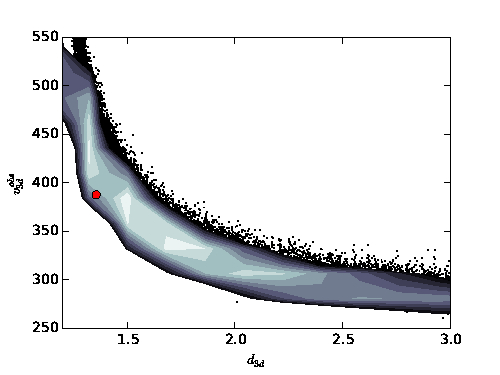
\includegraphics[scale=0.4]{./d_3d-vs-v_3dcol.jpg}
  \caption{Distribution of posterior probability in the 3D distance (Mpc) and 
   3D velocity (Km/s) space for a simulated merging cluster, red dot indicates the real current values.
   Others kinematical parameters like Time since Collision or velocity at the merger time are also well 
   recovered.}
 \end{figure}
}
\frame{
 \frametitle{Future Work}
 Study the physics properties of the galaxies that belong to the identified substructures, ordering
 them in a temporal line by the merger state.
}
\frame{
 \frametitle{Future Work}
 Construct a catalog of relaxed clusters in order to study the dark matter equation of state (Serra \& Dominguez 2011).
}


\frame{ 
\begin{figure}[h!]
 \centering
 
\includegraphics[scale=0.4]{./gracias.png}
 % gracias.png: 657x518 pixel, 72dpi, 23.18x18.27 cm, bb=0 0 657 518
\end{figure}
}
\end{document}

